\icode{E-MK-SI-L2-260928-005}
``极限滑草''受到青少年的追捧。如图所示，某同学在滑草斜面上从\(O\)点由静止开始做匀加速直线运动，先后连续经过\(P\)、\(M\)、\(N\)三点，已知\(MN\)间的距离是\(PM\)的两倍，\(PM\)段的平均速度是\qty{6}{m/s}，\(MN\)的平均速度是\qty{12}{m/s}，则该同学经过\(M\)点时的瞬时速度为\paren[D]

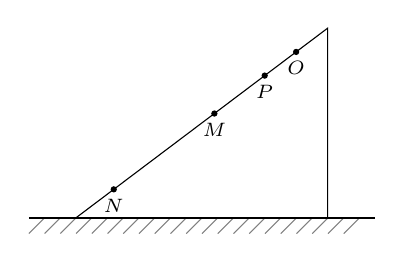
\begin{tikzpicture}[font=\scriptsize]
	\foreach \x in{-.6,-.4,...,3.6}
		\draw[gray] (\x,-.2)--++(.2,.2);
	\draw[thick] (-.6,0)--(3.8,0);
	\draw (0,0)--(37:4)--(37:4|-0,0);
	\foreach \r/\str in{3.5/O,3/P,2.2/M,.6/N}
		\fill (37:\r)node[below]{\(\str\)} circle(.04);
\end{tikzpicture}
\begin{choices}
	\item \qty{12}{m/s}
	\item \qty{11}{m/s}
	\item \qty{10}{m/s}
	\item \qty{9}{m/s}
\end{choices}
\begin{answer}
	D\qquad 提示：\(PM\)段和\(MN\)段时间相等
\end{answer}